% 
% Annual Cognitive Science Conference
% Sample LaTeX Paper -- Proceedings Format
% 

% Original : Ashwin Ram (ashwin@cc.gatech.edu)       04/01/1994
% Modified : Johanna Moore (jmoore@cs.pitt.edu)      03/17/1995
% Modified : David Noelle (noelle@ucsd.edu)          03/15/1996
% Modified : Pat Langley (langley@cs.stanford.edu)   01/26/1997
% Latex2e corrections by Ramin Charles Nakisa        01/28/1997 
% Modified : Tina Eliassi-Rad (eliassi@cs.wisc.edu)  01/31/1998
% Modified : Trisha Yannuzzi (trisha@ircs.upenn.edu) 12/28/1999 (in process)
% Modified : Mary Ellen Foster (M.E.Foster@ed.ac.uk) 12/11/2000
% Modified : Ken Forbus                              01/23/2004
% Modified : Eli M. Silk (esilk@pitt.edu)            05/24/2005
% Modified : Niels Taatgen (taatgen@cmu.edu)         10/24/2006
% Modified : David Noelle (dnoelle@ucmerced.edu)     11/19/2014

%% Change "letterpaper" in the following line to "a4paper" if you must.

\documentclass[10pt,letterpaper]{article}

\usepackage{cogsci}
\usepackage{commath}
\usepackage{graphicx}
\usepackage{pslatex}
\usepackage{siunitx}
\usepackage{apacite}


\title{TODO title}
 
\author{{\large \bf Jan Gosmann (jgosmann@uwaterloo.ca)} \\
  %Department of Psychology, 1202 W. Johnson Street \\
  %Madison, WI 53706 USA
  \AND{\large \bf Aaron Voelker (TODO)} \\
  \AND{\large \bf Chris Eliasmith (TODO)}
  %Department of Educational Psychology, 1025 W. Johnson Street \\
  %Madison, WI 53706 USA}
  }


\begin{document}

\maketitle


\begin{abstract}
    TODO

\textbf{Keywords:} TODO add your choice of indexing terms or keywords; kindly 
use a
semicolon; between each term
\end{abstract}


\section{Introduction}
Winner-take-all (WTA) mechanisms are often employed in cognitive 
models~\cite<e.g.,>{oreilly1998}.  A WTA mechanism receives a $d$-dimensional 
input of utility values for $d$ different choices. The output is supposed to be 
larger than zero for the dimension with highest utility and zero for all other 
inputs.

A large body of literature exists examining the optimality of WTA mechanisms and 
their consistency with neurobiological and psychological 
data~\cite<e.g.,>{bogacz2006,gold2007,smith2004}.  Here, however, we will 
investigate the suitability of two different WTA mechanisms in the context of 
large-scale cognitive modelling with spiking neurons on a set of benchmarks that 
are more normative in nature.  The first mechanism is an implementation of the 
leaky, competing accumulator model by~\citeA{usher2001}.  It has been widely 
used, for example in versions of the Temporal Context 
Model~\cite{sederberg2008}, and some of our models~\cite<e.g.,>{kajic2017}. We 
will compare this to an independent accumulator model with a second thresholding 
layer with recurrent connections to the first layer.  In both cases we are 
especially interested in situations with more than two choices ($d > 2$).

For the implementation of these models we use the Neural Engineering 
Framework~\cite<NEF;>{eliasmith2003} which allows us to directly implement the 
prescribed dynamics with spiking neurons. The NEF has been used in a wide range 
of models, including the largest functional brain model 
Spaun~\cite{eliasmith2012}.  We will give a short introduction to the NEF first, 
then describe the implementation of the two WTA mechanisms. Then we give the 
results on a number of metrics, followed by a discussion.

\section{Methods}

\subsection{The Neural Engineering Framework}
We employ the Neural Engineering Framework~\cite<NEF;>{eliasmith2003} which 
allows us to implement equations describing the model dynamics in spiking neural 
networks based on three principles: \emph{representation}, 
\emph{transformation}, and \emph{dynamics}.

\subsubsection{Principle 1: Representation}
The representation of a value $x(t)$ with a population of neurons is defined by 
the encoding and decoding. The encoding converting the value $x$ into a spike 
train or instantaneous firing rate $a_i(t)$ for neuron $i$ is given by
\begin{equation}
    a_i(t) = G_i\left[\alpha_i x(t) + J_i^{\mathrm{bias}}\right]
\end{equation}
where $\alpha_i$ is a gain factor, $J_i^{\mathrm{bias}}$ a bias current and 
$G_i$ is the neuron non-linearity. Here, we use spiking, leaky 
integrate-and-fire neurons as $G_i$.

Decoding weights $d_i$ are used to decode a value $\hat x(t)$ from such 
a population of neurons with
\begin{equation}
    \hat x(t) = \sum_i d_i \left[a_i(t) * h(t)\right]
\end{equation}
where $h(t) = \tau_{\mathrm{s}}^{-1}\exp(1/\tau_{\mathrm{s}})$ is an exponential 
synaptic filter with time constant $\tau_{\mathrm{s}}$.  The decoding weights 
are obtained with a least-squares optimization of the error $E_x = \abs{x 
    - \hat{x}}$.

For the transmission of a value from one population to another, the connection 
weights are given by
\begin{equation}
    W_{ij} = \alpha_j d_i \text{.}
\end{equation}

\subsubsection{Principle 2: Transformation}
By finding alternate decoding weights $d^f_i$ with the error given by $E_{f(x)} 
= \abs{f(x) - \hat x}$ arbitrary linear and non-linear functions $f(x)$ can be 
approximated in the connections between neural populations.

\subsubsection{Principle 3: Dynamics}
TODO

\subsection{Leaky, competing accumulator model}
We implement the widely used, leaky, competing accumulator (LCA) model proposed 
by~\citeA{usher2001}.  The dynamics for the state variables $x_i,\ i < N$, where 
$N$ is the number of choices, are given by:
\begin{equation} \label{eqn:usher-mcclelland}
    \begin{split}
        \frac{{\partial x}_i}{\partial t} &= \left(\rho_i - kx_i - \beta \sum_{j \neq i} x_j\right) \frac{1}{\tau} \\
        x_i &\rightarrow \max(x_i, 0) ,
    \end{split}
\end{equation}
where $\rho_i$ is the external input, $k$ is the leak rate, $\beta$ the lateral 
inhibition, and $\tau$ the time constant.
We set $k = \beta = 1$, since this will guarantee that the winning state converges to the value of its input, while the losing states converge to zero.
Other choices of $k$ merely alter the effective $\tau$ and the effective gain on the input, while other choices of $\beta$ will produce unwanted behaviour (see supplementary analysis).

Equation~\ref{eqn:usher-mcclelland} can easily be implemented with the NEF by 
using one population of neurons for each $x_i$.  We believe this implementation 
to be novel as it it does not treat the $x_i$ as neural firing rates, rather the 
neural firing rates are weighted by the decoding weights to precisely implement 
the stated dynamics. As such the model equations do not impose restrictions on 
the neuron model or requires to lump the neurons into a single population firing 
rate. This allows us to use biologically more realistic neurons while at the 
same time adhering to the dynamics prescribed by the model.  
Figure~\ref{fig:usher-mcclelland} shows an example output.
\begin{figure}
    \centering
    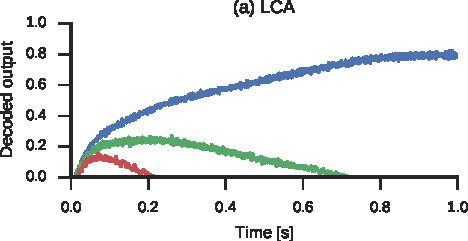
\includegraphics{figures/usher-mcclelland}
    \caption{Example time course of the state variables in the leaky, competing 
        accumulator model with three dimensions. The vector of inputs is given 
        by $(0.8, 0.7, 0.6)$.}\label{fig:usher-mcclelland}
\end{figure}

\subsection{Independent accumulator model}
The other investigated winner-take-all mechanism is an independent accumulator 
(IA) model, i.e.~there is no interaction like mutual inhibition among the 
accumulators. Compared to prior similar models (TODO refs), however, we add 
a second layer of independent, non-recurrent populations that get input from the 
first layer in a one to one projection. We decode the shifted Heaviside function 
$\bar{x}_{2,i} = \Theta(x^2_i - \vartheta)$ from it where $\vartheta = 0.8$ is 
a threshold value controlling how much evidence needs to be accumulated to 
produce an output.
The Heaviside decoded output of layer 2 projects back to layer 1 to add 
$\bar{x}_{2,i} - \bar{\beta} \sum_{j \neq i} \bar{x}_{2,j}$ to the input of $x_{1,i}$.
For $\bar{\beta} = 2$ (see supplementary analysis), the correct choice will self-excite while all other state variables will be 
suppressed once one of the accumulators reaches the threshold $\vartheta$.  The 
dynamics are described by the following equations:
\begin{equation}
    \begin{split}
        \frac{{\partial x}_{1,i}}{\partial t} &= \lambda \rho_i \frac{1}{\tau_1} + \left( 
            \bar{x}_{2,i} - \bar{\beta} \sum_{j \neq i} \bar{x}_{2,j} \right) \frac{1}{\tau_2} \\
        x_{1,i} &\rightarrow \max(x_{1,i}, 0) .
    \end{split}
\end{equation}

Instead of controlling the threshold $\vartheta$, in the context of the NEF, it 
is more convenient to keep $\vartheta$ fixed and scale the input with the 
$\lambda$ parameter. Mathematically both approaches are equivalent. We set 
$\lambda = 1$ where not noted otherwise. As the LCA model does not have 
a threshold parameter, we do not introduce the input scaling $\lambda$ in that 
model.  Figure~\ref{fig:indacc} shows an example of the model dynamics.
\begin{figure}
    \centering
    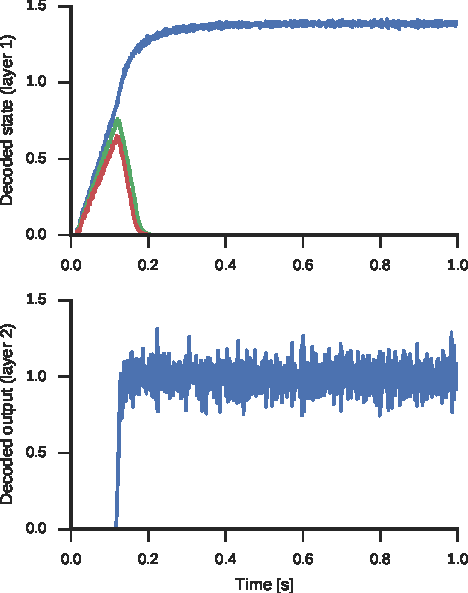
\includegraphics{figures/indacc}
    \caption{Example time course of the state variables $x_{1,i}$ and decoded 
        output $\bar{x}_{2,i}$ in the independent accumulator model with three 
        dimensions. The vector of inputs is given by (0.8, 0.7, 0.6).
    }\label{fig:indacc}
\end{figure}

\subsection{Metrics}
To test and compare the two WTA mechanisms we provide an input of $\rho_i 
= u - s \delta_{1i} + \eta_i$ where $u$ is the strength of the strongest input, 
$s$ the target separation to all other inputs, $\delta$ the Kronecker delta, and 
$\eta_i$ Gaussian white noise with standard deviation $\sigma$. Thus, without 
loss of generality, the first state variable receives the strongest input and 
all other state variables receive input that is smaller by $s$. We chose this 
input as for $\rho_i \rightarrow 0$ the influence of input $\rho_i$ will 
decrease and the effective number of choices to decide between would decrease  
As $s \rightarrow 0$ the problem gets more difficult. We will use $u = 1$ as 
long as not indicated otherwise and set the number of dimension to $d = 10$.  In 
both WTA models we use 200 neurons for each dimensions. In the IA network this 
are split as 150 neurons for each layer 1 population and 50 neurons for each 
layer 2 population. Further parameters are summarized in Table~\ref{tbl:params}.
\begin{table}
    \caption{Summary of parameter values.}\label{tbl:params}
    \begin{tabular}{ll}
        LCA time constant & $\tau = \SI{0.1}{\second}$ \\
        LCA recurrent parameters & $k = \beta = 1$ \\
        IA accumulation time constant & $\tau_1 = \SI{0.1}{\second}$ \\
        IA feed-back time constant & $\tau_2 = \SI{0.1}{\second}$ \\
        IA threshold & $\vartheta = 0.8$ \\
        IA recurrent parameters & $\lambda = 1, \bar{\beta} = 2$ \\
        Recurrent synaptic time constant & $\tau_{\mathrm{s}} 
        = \SI{0.1}{\second}$ \\
        Feed-forward synaptic time constant & $\tau_{\mathrm{s}} 
        = \SI{0.005}{\second}$ \\
        Output decoding synaptic time constant & $\tau_{\mathrm{s}} 
        = \SI{0.01}{\second}$
    \end{tabular}
\end{table}

To evaluate the two mechanisms on this input, we use a number of metrics. First 
we determine whether the model is able to form a clear decision at all within 
a second of simulated time. To count as a clear decision, at least one output 
needs to stay above 0.15 for the time interval
$]\SI{1}{\second}, \SI{2}{\second}]$. % chktex 10
This lower bound was chosen to ensure that noise on a zero output is not 
mistaken as a non-zero output.  Furthermore, we require that the largest output 
will be the largest output for all of the time interval or in other words the 
decision does not change during that time interval.

This does not take into account whether the winning output actually corresponds 
to the strongest input, but sometimes it can be more desirable to produce 
a clear decision than actually finding the strongest input in all instances. In 
other situations, though, the correctness of the decision might be of higher 
importance. We consider a trial correct if the model forms a clear decision and 
the largest output corresponds to the largest input. All remaining metrics will 
be calculated on the subset of trials with a clear decision.

The time it takes to form a decision can be relevant too.  We define the 
decision time as how long it takes to fulfill the conditions of a clear 
decision.

These metrics cover the basic performance of the WTA mechanisms. When using 
a WTA mechanism within larger cognitive models, the exact magnitude of the 
outputs can be important. Ideally, the output would be 1 for the winner and zero 
for all other outputs.\footnote{Technically, the winner output could be scaled 
    to any magnitude. We use 1 here as it is most convenient to work with.} The 
LCA dynamics, however, prescribe an output of $u$ for the winner with $u$ being 
the largest input. We define the \emph{winner error} $E_1$ as the difference of 
the winner output from $u$ for the LCA model, as the difference from 1 for the 
IA model and, for both models, the \emph{runner-up error} $E_2$ as the 
difference of second largest output from 
0 (negative values treated as 0). We use the average output values of the time 
  interval
 $]\SI{1}{\second}, \SI{2}{\second}]$ % chktex 10
to calculate these error values as the values fluctuate over time.

These two metrics only look at the final output averaged over time, but the 
model can produce transient outputs before the final decision is achieved.  
Within the context of a larger model, this can be a problem as the transient 
output could already be interpreted as a decision. Thus, we define $E_{2,\max}$ 
as the highest output of a non-winning output during the whole simulation.

\section{Results}
We find that the ability to reach a clear decision depends on the magnitude of 
the highest input for both networks. This is not surprising. In the LCA model 
the output magnitude will be determined by the input magnitude of the largest 
input.  As such the largest input needs to be above 0.15 to fulfill the 
requirements. For the independent accumulator model the input has to be large 
enough to reach the integration threshold within the time limit. By increasing 
the input scaling $\lambda$ or the time limit one could get a clear decision for 
smaller inputs within the time limit. We further find that the IA model is 
independent of the input noise and target separation for all tested parameters.  
This is not the case for the LCA model as shown in Figure~\ref{fig:decisions} 
where the fraction of trials without a clear decision increases with noise and 
smaller target separation.
\begin{figure}
    \centering
    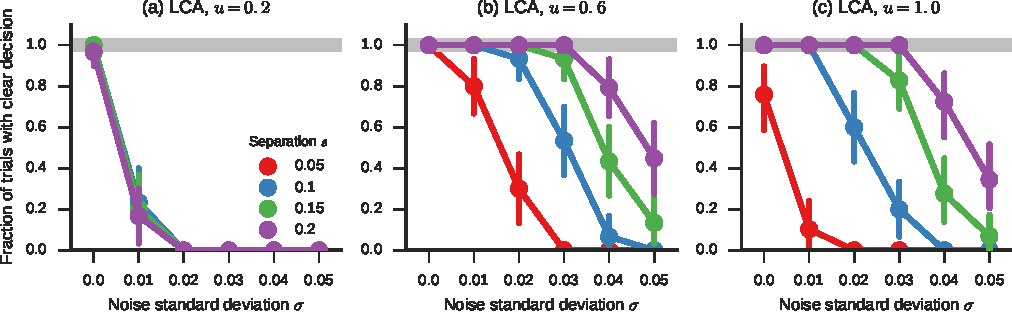
\includegraphics{figures/decisions}
    \caption{Fraction of trials with a clear decision for different input noise 
        standard deviations $\sigma$ and target separations $s$ for the LCA 
        model. Error bars denote bootstrapped 95\% confidence intervals.  The 
        grey horizontal line shows the optimum.}\label{fig:decisions}
\end{figure}

However, when considering the correctness of the decisions (see 
Fig.~\ref{fig:correct}) the LCA model is doing better. We can alleviate that 
difference to some degree by reducing the input scaling to $\lambda = 0.2$, but 
perform still worse for some combinations of input noise and target separation 
when staying below the time limit. This in some part due to a systematic bias 
for certain dimensions introduced in the second layer of the IA model. In the 
NEF the neuron gain and bias parameters are usually picked from random 
distributions. As such the layer 2 populations will become active at slightly 
different thresholds. By using identical layer 2 populations, i.e.~identical 
gain and bias parameters for each population, this bias can be eliminated and 
the IA model performs better than the LCA model in most instances.
\begin{figure*}
    \centering
    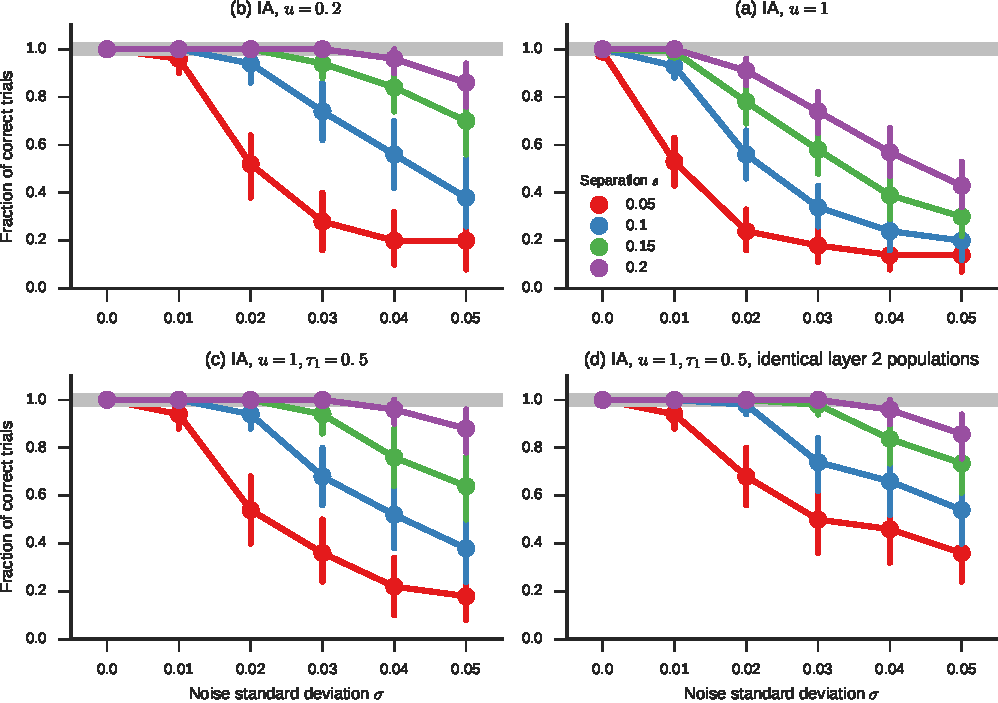
\includegraphics{figures/correct}
    \caption{Fraction of correct trials for different input noise standard 
        deviations $\sigma$, target separations $s$, and models.  Error bars 
        denote bootstrapped 95\% confidence intervals. The grey horizontal line 
        shows the optimum.}\label{fig:correct}
\end{figure*}

The time required to reach a decision in the LCA model depends mostly on the 
target separation and amount of noise on the input (see Fig.~\ref{fig:time}), 
the magnitude of the largest input is of minor influence. Also, the confidence 
intervals indicate a larger variance in the decision times with less target 
separation and more input noise. In contrast to that, in the IA model the scaled 
magnitude of the largest input is the most important factor.  Depending on this 
magnitude the network can either be faster or slower than the LCA network, but 
it will need more time to achieve the same fraction of correct responses.  There 
is also a slight influence of target separation and input noise with an 
interaction of these two parameters.
\begin{figure*}
    \centering
    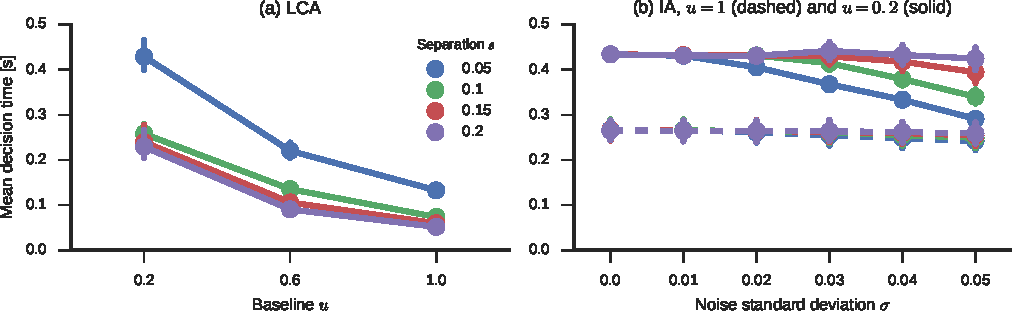
\includegraphics{figures/time}
    \caption{Mean decision times for different input noise standard deviations 
        $\sigma$ and target separations $s$ for the LCA and IA model. For the IA 
        model $u = 0.2$ is shown which shows the interaction of target 
        separation and input noise most clearly. Error bars denote bootstrapped 
        95\% confidence intervals.  The grey horizontal lines show the 
        optimum.}\label{fig:time}
\end{figure*}

The output of the IA model matches almost perfectly the specifications of 
producing an output of 1 for the winner and 0 for all other dimensions.  This is 
not the case for the LCA model (see Fig.~\ref{fig:error}).  For small target 
separations the output of the winner will stay below $u$ and this will get worse 
with increased noise. Furthermore, the LCA model will have residual outputs of 
non-winning choices under noisy conditions and with small target separations.
\begin{figure*}
    \centering
    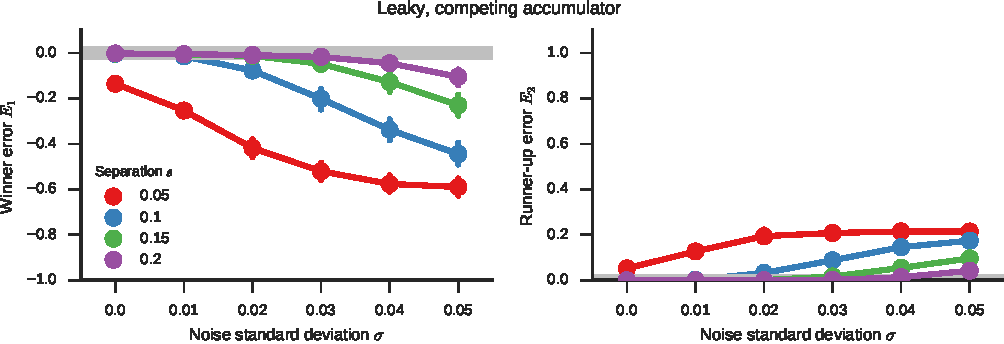
\includegraphics{figures/error}
    \caption{Error on outputs for different input noise standard deviations 
        $\sigma$ and target separations $s$ for the LCA model.  Error bars 
        denote bootstrapped 95\% confidence intervals. The grey horizontal lines 
        show the optimum.}\label{fig:error}
\end{figure*}

Finally, looking at the transient responses both models might produce outputs of 
non-winning choices (see Fig.~\ref{fig:transient}). For the LCA model these 
increase with noise on the input and, for small target separation, can approach 
the final output of the winning dimensions. For the IA model, transient outputs 
are smaller in noisy conditions, but can be higher than for the LCA model in 
less noisy conditions.  The magnitude of such transient responses is reduced by 
decreasing the input scaling.
\begin{figure*}
    \centering
    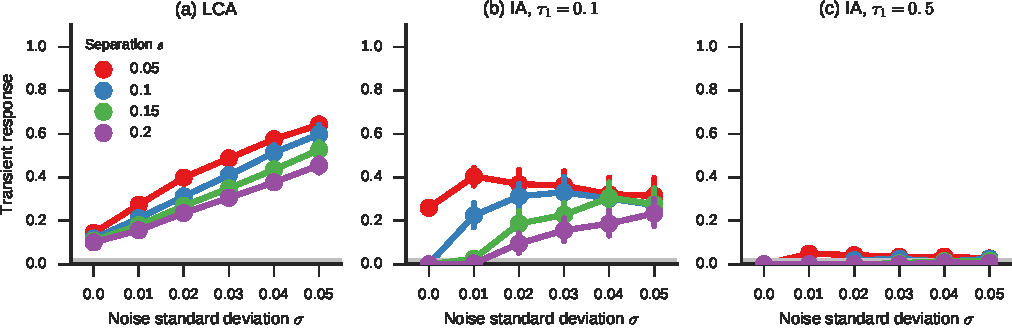
\includegraphics{figures/transient}
    \caption{Highest transient response of non-winning dimensions for different 
        input noise standard deviations $\sigma$ and target separations $s$ for 
        the LCA and IA model. Error bars denote bootstrapped 95\% confidence 
        intervals. The grey horizontal lines show the 
        optimum.}\label{fig:transient}
\end{figure*}

\section{Discussion}
We find neither of the two networks to perform better on all metrics, but rather 
they are suited for slightly different things. The leaky, competing accumulator 
model is better at quickly determining the correct winner. However, under noisy 
conditions it can end up not producing a clear output at all and thus failing to 
produce a decision.  The independent accumulator model might not be as quick or 
find the correct winner as often, but given enough time it will eventually 
arrive at a decision and produce a clear output.

The LCA network is especially suited for situations where a decision needs to be 
continuously adjusted. The prescribed dynamics essentially try to output what 
the currently largest input is considering some smoothing over time. This makes 
it quick to respond to changes of the input, but can also lead to random 
switching outputs due to noise. In comparison, the IA model is more suited in 
situations where a discrete sequence of decisions is required.  During the 
initial phase the model will just integrate evidence without any output and 
after making a decision, it is necessary to reset the model by inhibiting all 
layer 1 neurons. This limits the how quickly successive decisions can be made, 
but at the same time, once a decision is made, the network provides a stable 
output.

There are also certain considerations to be made when integrating these networks 
into larger neural or cognitive models. This integration is easy for the IA 
model as it provides a clear output. The output of the winning choice is also 
always close to one, independent of the input, which makes it easy to detect 
when the decision has been made and processing can continue. This is problematic 
in the LCA model where we get a fluctuating output before the final decision and 
the magnitude of the output depends on the input magnitude. This makes it 
problematic to use a fixed threshold to detect the decision. Furthermore, 
transient responses of non-winning dimensions can get close to the final output 
of the winning dimension in the LCA model.

Part of the reason why the independent accumulator model produces less correct 
responses is the systematic bias introduced in the second layer. By eliminating 
this bias through identical ensembles the correctness of the model is increased 
considerably. However, this would require a very precise tuning of the neurons 
that might not be biologically plausible.

One critique of non-leaky accumulator models is that their ability to 
discriminate the largest input increases indefinitely with time (TODO~ref) and 
that there is no sensible stopping criterion. However, this assumes that the 
time to reach a decision has no cost. If that time has a cost, the cost of 
spending more time on the decision will at some point exceed the gain by making 
a correct decision. Furthermore, this argument assumes integration with perfect 
accuracy. But in a neural network resources are limited, as such the range and 
accuracy of values that can be represented in a neural population is limited.  
At some point this would counterbalance any additional evidence.

We did not investigate the biological plausibility here because this has been 
done before for different WTA networks.  Also, the implementation in spiking 
neurons ensures a certain level of biological plausibility. We also did not look 
at at the influence of the number of dimensions $d$ in detail, but qualitatively 
the results will stay the same. For higher $d$, we expect less correct responses 
as each additional dimensions adds a chance that this dimension will win out due 
to noise.

TODO\@: looking only at cases where a decision could be made within the results, 
include a number of parameters and github url.

\section{Notes}
Simulation source code and additional analysis results are available at 
\url{https://github.com/ctn-waterloo/cogsci17-decide}.  These have not been peer 
reviewed.

\section{Acknowledgments}
TODO anything missing here?
This work was supported by the Canada Research Chairs program,
the NSERC Discovery grant 261453, Air Force Office of Scientific Research grant 
FA8655-13-1-3084, CFI and OIT\@.  % chktex 8


\bibliographystyle{apacite}

\setlength{\bibleftmargin}{.125in}
\setlength{\bibindent}{-\bibleftmargin}

\bibliography{references}


\end{document} % chktex 17
